\chapter{Experiments}\label{sec:exps}{}
In this section, we present the details of the experiment setups and the corresponding results. To illustrate the effectiveness of our proposed model, we compare it with some strong baselines on sequential recommendation task. Moreover, we have published our reproductive code\footnote{https://bit.ly/2WZWTKC}.

We start with three research questions (RQ) to lead the experiments and the following discussions.
\begin{itemize}
	\item [\textbf{RQ1}] Compared to the baseline models, does SCoRe achieve state-of-the-art performance in sequential recommendation task?
	\item [\textbf{RQ2}] What is the influence of different components in~\score? Is the sampling method described in Section~\ref{sec:sampling} useful?
	\item [\textbf{RQ3}] What patterns does the proposed model capture for the final recommendation decision?
\end{itemize}

\section{Experimental Setups}
In this part, we describe our experiment setups including datasets with preprocessing method, some important implementation details, evaluation metrics and the compared baselines.
\subsection{Datasets}
We use three real-world large-scale datasets to evaluate all the compared models. The dataset statistics have been shown in Table ~\ref{tab:dataset-statistics}.
\begin{description}[leftmargin=15pt]
	\item [CCMR] \cite{cao2016complete} is a dataset consists of movie rating logs collected from Douban, which is one of China's largest movie review websites. The data is collected and dumped in May 2015.
	\item [Tmall] \footnote{https://tianchi.aliyun.com/dataset/dataDetail?dataId=42} is provided by Alibaba Group which contains user behavior history on Tmall e-commerce platform from May 2015 to November 2015.
	\item [Taobao] \cite{zhu2018learning} is a dataset consisting of user behavior data collected from Taobao\footnote{https://tianchi.aliyun.com/dataset/dataDetail?dataId=649}, one e-commerce platform in China. It contains user behaviors from November 25 to December 3, 2017 of several behavior types including click, purchase, add to cart and item favoring.
\end{description}

\noindent\textbf{Dataset Preprocessing}.
As we consider the user-item interactions as a sequence of bipartite graphs, we cut it into total $T$ time slices with the same time interval as shown in Table~\ref{tab:dataset-statistics}. And for each time slice, we use the interaction records within it to construct the user-item bipartite graph.
In every sliced graph, we start from the target user/item node and step out for $K$ hops to get the \textit{user/item-rooted interaction set} and the interaction sets of every time slice form the user/item-side sequences. 
We set $K=2$ for the three datasets.

\begin{table}[t]
	%	\scriptsize
	\centering
	\caption{The dataset statistics.}\label{tab:dataset-statistics}
	%	\vspace{-10pt}
	\resizebox{\columnwidth}{!}{
		\begin{tabular}{c|r|r|r|r|r}
			\hline
			Dataset & Users \# & Items \# & Interaction \# & Time slices \# & Time interval $\Delta T$\\
			\hline
			CCMR & 4,920,695 & 190,129 & 283,775,314 & 41 & 90 days\\
			\hline
			Tmall & 424,170 & 1,090,390 & 54,925,331 & 13 & 15 days\\
			\hline
			Taobao & 987,994 & 4,162,024 & 100,150,807
			 & 9 & 1 day\\
			\hline
		\end{tabular}
	}
%	\vspace{-10pt}
\end{table}

% \jiarui{add figures about how many 1-hop/2-hop neighbor a user/item has at each time slice, ccmr vs taobao/tmall item side differences}

\noindent\textbf{Positive \& Negative Samples}.
To evaluate the recommendation performance, we use one positive item and sample 100 negative items at the prediction time $T + 1$ for each user in all three datasets.
For Tmall and Taobao datasets, as we only have the positive user feedbacks (click, buying, etc.), we have to randomly sample the negative items. As for CCMR datasets, we regard items whose ratings are 5 or 4 as positive items and those whose ratings are 1,2 or 3 as negative items. If a user does not have enough negative items, we use random sampling to generate negative items for her.

\noindent\textbf{Train \& Test Splitting}.
The training set contains the sequential behaviors from 1st to $(T-1)$th time slice, we use the interactions history from 1 to $T-2$ to predict the interactions in $(T-1)$. For the testing set, we use the interactions data from 1 to $T-1$ to predict the interactions in $T$.

\noindent\textbf{Implementation Details}.
It is common that the target user doesn't have any interaction record in a time slice, and similarly, the target item may be not visited by any user in a time slice. To handle this issue, we use a unified embedding vector to represent these users and items.

We set the size of all the k-hop \textit{user/item-rooted interaction sets} to $S$ which can be regarded as a hyperparameter.
For each hop's neighbors, we follow the sampling strategy described in Section~\ref{sec:sampling}.% and the sampling happens for every data sample when it is fed to the model which means it could be different nodes in \textit{user/item-rooted interaction set} for the same data sample during training.


\subsection{Evaluation Metrics}
Three evaluation metrics are used and all of them are widely used in recommendation tasks.

\textbf{HR@k} (\textit{Hit Ratio@k}) measures the proportion of samples that the positive item is among the top-k in all test cases which is computed as,
\begin{equation}
HR@k = \frac{1}{|\mathcal{U}|} \sum_{u \in \mathcal{U}} \mathbb I (R_{u, v} \leq k),
\end{equation}
where $R_{u,v}$ is the ranking position of the user $u$'s interacting with item $v$, and $\mathbb I$ is the indicator function.

\textbf{NDCG@k} (Normalized Discounted Cumulative Gain) is a position-aware metric which assigns larger weights on higher ranks of the positive item, which is calculated as,
\begin{equation}
NDCG@k = \frac{1}{|\mathcal{U}|} \sum_{u \in \mathcal{U}} \frac{2^{\mathbb I (R_{u, v} \leq k)} - 1} {log(R_{u, v} + 1)}.
\end{equation}

\textbf{MRR} (Mean Reciprocal Rank) is another position-aware metric that is calculated as,
\begin{equation}
MRR = \frac{1}{|\mathcal{U}|} \sum_{u \in \mathcal{U}} \frac{1}{R_{u, v}}.
\end{equation}

% Because we just have one positive item per user, HR@k is equal to Recall@k and it is linear to Precision@k, while MRR is equal to Mean Average Precision (MAP). 
As HR@1 is equal to NDCG@1, so in this work, we report HR@\{1,5,10\}, NDCG@\{5,10\} and MRR in detail.

 
\subsection{Compared Baselines}\label{sec:comp-models}
To illustrate the effectiveness of our model, we compare \score ~with two CF models, three sequential recommendation models and two graph-based models.
We follow \cite{zhou2018deepb} that all the models take the input sparse features and feed them through an embedding layer for the subsequent inference.

The first group of models are CF models:
\begin{itemize}[leftmargin=40pt]
	\item [\textbf{SVD++}] \cite{koren2008factorization} is a hybrid method of latent factor model and neighbor-based model which is the fundamental approach of collaborative filtering recommendation. It regards all the sequential behaviors as a whole and ignores the temporal dynamics.
	\item [\textbf{DELF}] \cite{cheng2018delf} is the state-of-the-art CF method which utilizes deep neural networks to capture complex non-linear interaction patterns from both user-side and item-side.
\end{itemize}

The second group is sequential recommendation methods, which are based on RNNs, CNNs, or Transformer architecture:
\begin{itemize}[leftmargin=40pt]
	\item [\textbf{GRU4Rec}] \cite{hidasi2015session} bases on GRU and it is the first work using the recurrent cell to model sequential user behaviors.
	\item [\textbf{Caser}] \cite{tang2018personalized} is based on CNNs that uses horizontal and vertical convolutional filters to capture user behavior patterns at different scales.
	\item [\textbf{SASRec}] \cite{kang2018self} bases on Transformer \cite{vaswani2017attention}, it only uses self-attention mechanism without recurrent architecture. It achieves very competitive performance in sequential recommendation task.
\end{itemize}

The third group is graph-based sequential recommendation models. For fair comparison, we use the same time interval to do time slicing.
\begin{itemize}[leftmargin=40pt]
	\item [\textbf{RRN}] \cite{wu2017recurrent} is the first RNN-based model that considers both the user- and item-side sequence. It uses sum-pooling to aggregate the information inside a time slice which can be regarded as a graph-based model.
	\item [\textbf{GCMC}] \cite{fadel2018link} is a link prediction model based on sequential bipartite graph for recommender system. It uses graph structured data for final prediction. GCMC is a method for matrix completion using Graph Convolutional Networks (GCNs) to handle dynamic graphs. 
	\item [\textbf{SCoRe}] is our proposed model which is described in Section~\ref{sec:method}.
\end{itemize}

\begin{table}[t]
	%	\scriptsize
	\centering
	\caption{The hyperparameter settings of \score. $h$ is hidden vector size. $\eta$ is learning rate, $b$ is batch size.}\label{tab:hyperparas}
	%	\vspace{-10pt}
	\resizebox{0.9\columnwidth}{!}{
		\begin{tabular}{c|l}
			\hline
			CCMR & $d=16$, $h=32$, $K=2$, $S=5$, $\eta=0.0005$, $b=100$, $\lambda=0.005$\\
			Tmall & $d=16$, $h=32$, $K=2$, $S=10$, $\eta=0.001$, $b=200$, $\lambda=0.0005$\\
			Taobao & $d=16$, $h=32$, $K=2$, $S=10$, $\eta=0.001$, $b=200$, $\lambda=0.0001$\\
			\hline
		\end{tabular}
	}
	\vspace{-10pt}
\end{table}

\subsection{Hyperparameter Settings}
The hyperparameters are determined by optimizing MRR on test set. The detailed hyperparameters of \score~ are listed in Table~\ref{tab:hyperparas}. For fair consideration, the latent dimension of all compared baselines remain the same, while the other hyperparameters of all the baselines are set based on grid search in the same search space.


\begin{table*}[h]
	\centering
	\caption{Performance comparison against baseline models. Bold values are the best in each row, while the second best values are underlined. Improvements over baselines are statistically significant with $p$ < 0.01. HR, NDCG, MRR: the higher, the better)}\label{tab:perf-table}
	\tiny
	\resizebox{0.9\textwidth}{!}{
		\begin{tabular}{c|c|cc|ccc|ccc}%ccc|ccc}
			\hline
			\multirow{2}{*}{Dataset} & \multirow{2}{*}{Metric} & \multicolumn{2}{c|}{Group 1} & \multicolumn{3}{c|}{Group 2} & \multicolumn{3}{c}{Group 3}\\
			& & SVD++ & DELF & GRU4Rec & Caser & SASRec & RRN & GCMC & \score\\
			\hline
			\multirow{6}{*}{CCMR} & HR@1 & 0.2378 & 0.6536 & 0.6703 & 0.6777 & \underline{0.6979} & 0.6633 & 0.6591 & \textbf{0.7001}\\
			& HR@5 & 0.4288 & 0.9087 & 0.8911 & 0.8907 & 0.9047 & 0.903 & \underline{0.9063} & \textbf{0.9118} \\
			& HR@10 & 0.5462 & 0.9586 & 0.9268 & 0.9184 & 0.9361 & 0.9469 & \underline{0.9508} & \textbf{0.9583} \\
			& NDCG@5 & 0.3356 & 0.7919 & 0.7917 & 0.7954 & \underline{0.8123} & 0.7957 & 0.7946 & \textbf{0.8161} \\
			& NDCG@10 & 0.3735 & 0.8084 & 0.8034 & 0.8045 & \underline{0.8226} & 0.8101 & 0.8092 & \textbf{0.8281} \\
			& MRR & 0.3375 & 0.7617 & 0.7662 & 0.7699 & \underline{0.7878} & 0.7681 & 0.7652 & \textbf{0.7913} \\
			\hline
			\hline
			\multirow{6}{*}{Tmall} & HR@1 & 0.1229 & 0.2001 & 0.1979 & 0.2029 & 0.3312 & 0.4177 & \underline{0.4254} & \textbf{0.4764} \\
			& HR@5 & 0.3098 & 0.3765 & 0.3818 & 0.4037 & 0.6307 & \underline{0.6452} & 0.6449 & \textbf{0.6806} \\
			& HR@10 & 0.3438 & 0.4573 & 0.4713 & 0.4925 & 0.7072 & 0.7449 & \underline{0.7512} & \textbf{0.7632} \\
			& NDCG@5 & 0.2112 & 0.2975 & 0.2947 & 0.3089 & 0.4935 & 0.5368 & \underline{0.5403} & \textbf{0.5842} \\
			& NDCG@10 & 0.2342 & 0.3130 & 0.3236 & 0.3376 & 0.5184 & 0.5691 & \underline{0.5747} & \textbf{0.6109} \\
			& MRR & 0.1373 & 0.2990 & 0.2950 & 0.3058 & 0.4676 & 0.5257 & \underline{0.5314} & \textbf{0.5734} \\
			\hline
			\hline
			\multirow{6}{*}{Taobao} & HR@1 & 0.0705 & 0.1299 & 0.1117 & 0.1292 & 0.1897 & 0.2138 & \underline{0.2164} & \textbf{0.2431} \\
			& HR@5 & 0.1539 & 0.2999 & 0.3001 & 0.3022 & 0.3871 & \underline{0.4695} & 0.4672 & \textbf{0.4991} \\
			& HR@10 & 0.2063 & 0.4656 & 0.4395 & 0.4539 & 0.5331 & \underline{0.6213} & 0.6156 & \textbf{0.6467} \\
			& NDCG@5 & 0.0998 & 0.1719 & 0.1667 & 0.1724 & 0.2512 & 0.3447 & \underline{0.3449} & \textbf{0.3590} \\
			& NDCG@10 & 0.1082 & 0.2008 & 0.1995 & 0.2013 & 0.2788 & \underline{0.3937} & 0.3929 & \textbf{0.4112} \\
			& MRR & 0.0935 & 0.1203 & 0.1119 & 0.1232 & 0.2198 & 0.3402 & \underline{0.3411} & \textbf{0.3786} \\
			\hline
		\end{tabular}
	}
	% \vspace{-10pt}
\end{table*}

\section{Evaluation Results: RQ1} \label{sec:comp_results}
% \kan{the influence of sparsity in data is an issue. we should discuss about it.}

The experimental results are shown in Table~\ref{tab:perf-table}, we find several observations that:
\begin{itemize}[leftmargin=15pt]
	\item By comparing the performance of \score~ and other baseline models, it outperforms baselines by 134.5\% to 0.4\%, 317.6\% to 7.9\% and 304.9\% to 11.0\% on MRR in CCMR, Tmall and Taobao dataset, respectively. And it also shows significant improvements on the other metrics so \score~ achieves the state-of-the-art performance in sequential recommendation task.
	\item For the models in Group 1, they do not consider the temporal dynamics of user behaviors thus perform not so good as models in Group 2 and 3. DELF uses both user-side and item-side interaction information so it achieves better performance than SVD++ which only utilizes user-side information.
	\item By comparing the performance of Group 2 and 3, we find in Tmall and Taobao dataset that, Group 3 outperforms Group 2 over CCMR dataset, SASRec and Caser are better than Group 3. As shown in Table~\ref{tab:dataset-statistics}, Tmall and Taobao has a lot more items than CCMR, which makes ranking items more difficult in Tmall and Taobao. So it is more important on these two datasets to take item-side sequence into consideration because it gives the models more information than just using single user-side sequence. 
	\item SASRec achieves satisfactory performance, especially compared to the other models in Group 1/2. It is accounted for utilizing the effective self-attention mechanism and more supervision signals at each time point.
	\item GCMC performs better than RRN in many cases. It may because that RRN just simply apply sum-pooling over the neighbors' information at each time slice, while GCMC uses graph convolution network to better capture the neighbors' information.
\end{itemize}

\textbf{Influence from the size of \textit{user/item-rooted interaction set}}.
We vary the size of \textit{user/item-rooted interaction set} of each hop to further investigate the robustness of \score. The results are shown in Table~\ref{tab:size-perf-table}. 
We find that when size increases, the performance is improved at first because that the larger the size is, the more information it contains. And when the size continues to increase, the performances begin to drop which indicates that too much noise and useless information is introduced.

\begin{table}[h]
	\centering
	\caption{Performance comparison on different size of \textit{user/item-rooted interaction set.}}\label{tab:size-perf-table}
	\tiny
	\resizebox{0.9\columnwidth}{!}{
		\begin{tabular}{c|c|cccc}
			\hline
			\multirow{2}{*}{ Dataset } & \multirow{2}{*}{ Metric } & \multicolumn{4}{c}{ Size of Interaction Set } \\
			& & 5 & 10 & 15 & 20 \\
			\hline
			\multirow{3}{*}{ CCMR } & HR@10 & \textbf{0.9583} & 0.9555 & 0.9498 & 0.9423 \\
			& NDCG@10 & \textbf{0.8281} & 0.8239 & 0.8232 & 0.8221 \\
			& MRR & \textbf{0.7913} & 0.7909 & 0.7895 & 0.7829 \\
			\hline
			\multirow{3}{*}{ Tmall } & HR@10 & 0.7589 & \textbf{0.7632} & 0.7619 & 0.7607 \\
			& NDCG@10 & 0.6091 & \textbf{0.6109} & 0.6087 & 0.6052 \\
			& MRR & 0.5658 & \textbf{0.5734} & 0.5698 & 0.5611 \\
			\hline
			\multirow{3}{*}{ Taobao } & HR@10 & 0.6288 & \textbf{0.6467} & 0.6319 & 0.6299 \\
			& NDCG@10 & 0.4068 & \textbf{0.4112} & 0.4081 & 0.4027 \\
			& MRR & 0.3679 & \textbf{0.3786} & 0.3673 & 0.3648 \\
			\hline
		\end{tabular}
	}
	\vspace{-10pt}
\end{table}


\section{Ablation Study: RQ2} \label{sec:ab-study}
In this section, we conduct some ablation studies to investigate the effectiveness of four important components of \score~: (1) \textit{Interactive Attention Mechanism} in dual sequences modeling; (2) \textit{Co-Attention Graph Network} for spatial information aggregation; (3) The consideration of using multi-hop instead of just one hop. (4) The importance sampling strategy which is used to find more relevant neighbors and reduce noise.

%\begin{figure}[h]
%	\centering
%	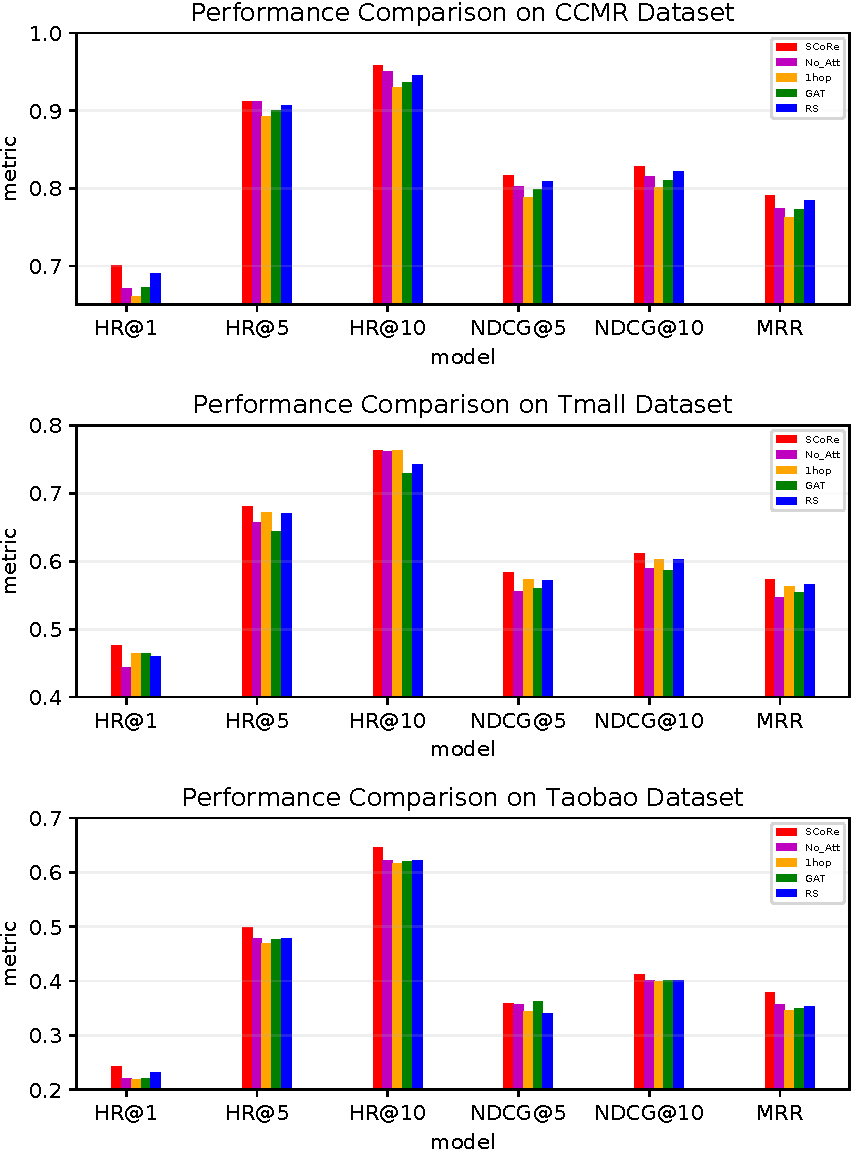
\includegraphics[width=0.9\columnwidth]{figures/ab_study.pdf}
%	\caption{Performance Comparison of Ablation Study.}
%	\label{fig:ab_study}
%	\vspace{-10pt}
%\end{figure}

\begin{table}[h]
	\centering
	\caption{Performance comparison of ablation study} \label{tab:ab_study_table}
	\tiny
	\resizebox{\columnwidth}{!}{
		\begin{tabular}{c|c|ccccc}
			\hline
			\multirow{2}{*}{ Dataset } & \multirow{2}{*}{ Metric } & \multicolumn{5}{c}{ models }\\
			& & RIA & Single-hop & GAT & RS & \score \\
			\hline
			\multirow{3}{*}{ CCMR } & HR@10 & 0.9509 & 0.9296 & 0.9358 & 0.9452 & \textbf{0.9583} \\
			& NDCG@10 & 0.8157 & 0.8011 & 0.8104 & 0.8217 & \textbf{0.8281} \\
			& MRR & 0.7741 & 0.7621 & 0.7724 & 0.7841 & \textbf{0.7913} \\
			\hline
			\multirow{3}{*}{ Tmall } & HR@10 & 0.7620 & 0.7632 & 0.7287 & 0.7431 & \textbf{0.7632} \\
			& NDCG@10 & 0.5893 & 0.6029 & 0.5866 & 0.6032 & \textbf{0.6109} \\
			& MRR & 0.5567 & 0.5633 & 0.5543 & 0.5662 & \textbf{0.5734} \\
			\hline
			\multirow{3}{*}{ Taobao } & HR@10 & 0.6216 & 0.6172 & 0.6201 & 0.6212 & \textbf{0.6467} \\
			& NDCG@10 & 0.4001 & 0.3991 & 0.4017 & 0.4015 & \textbf{0.4112} \\
			& MRR & 0.3575 & 0.3456 & 0.3498 & 0.3523 & \textbf{0.3786} \\
			\hline
		\end{tabular}
	}
%	\vspace{-10pt}
\end{table}


\begin{figure*}[h]
	\centering
	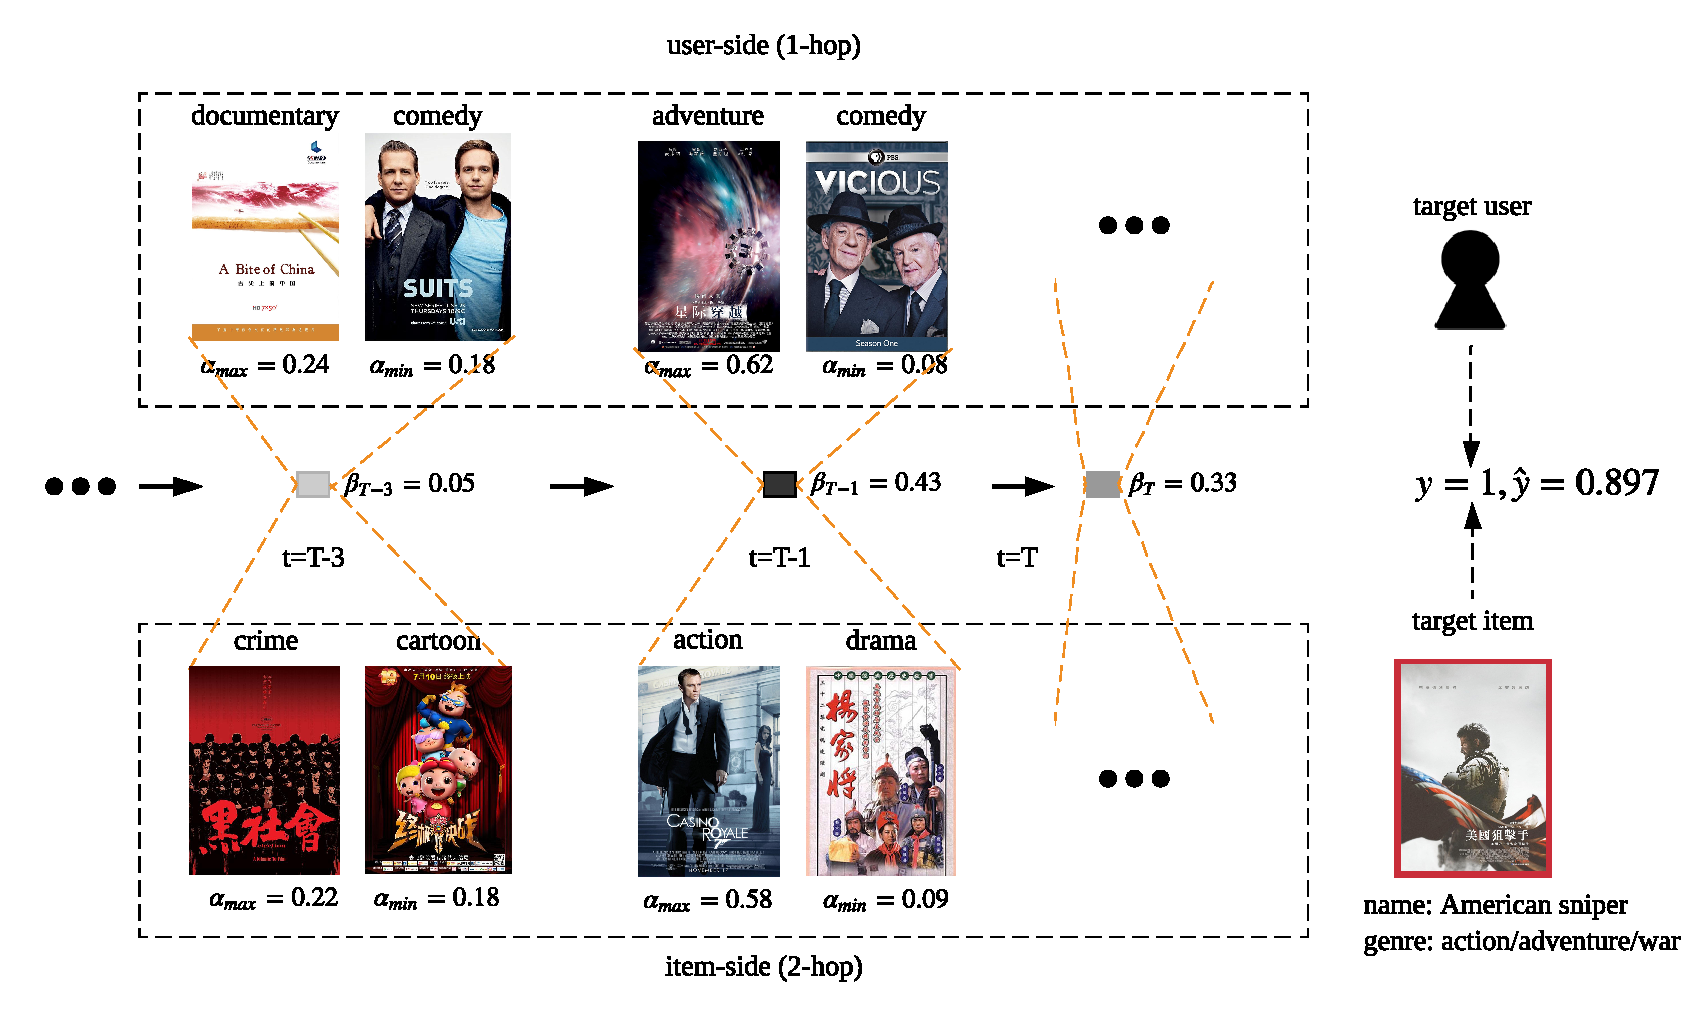
\includegraphics[width=0.8\textwidth]{visual.pdf}
	\caption{Visualization analysis of patterns that are captured by \score.}
	\label{fig:visual}
	\vspace{-10pt}
\end{figure*}

We set four comparative settings, and the performances of them have been shown in Table~\ref{tab:ab_study_table}.
The details of the four settings are listed as below.
\begin{itemize}[leftmargin=15pt]
	\item \textbf{RIA} (Remove Interactive Attention) removes the attention part described in~\ref{sec:attention} and set the final sequential representations of target user and item as $\bm r_u = h_T^u$ and $\bm r_v = h_T^v$ of Eq.~(\ref{eq:seq_rep}).
	\item \textbf{Single-hop} only uses the 1-hop neighbors of the target user and item that $\mg_t(u) = \mg^1_t(u)$ and $\mg_t(v) = \mg^1_t(v)$.
	\item \textbf{GAT} uses Graph Attention Network proposed in \cite{velivckovic2017graph}. We use this model to evaluate the effectiveness of the proposed \textit{Co-Attention Graph Network}.
	\item \textbf{RS} (Random Sampling) is the same as \score, but it uses random sampling instead of importance sampling described in Section~\ref{sec:sampling}.
\end{itemize}
Except for the changes mentioned above, the other parts of the models and experiment settings remain identical to that above to ensure fair comparison.

Except for the changes mentioned above, the other parts of the models and experimental settings remain identical to ensure the fairness of comparison.

From Table~\ref{tab:ab_study_table} we can find that (1) in CCMR and Taobao dataset, Single-hop performs worse than RIA and GAT but performs better than them in Tmall datasets. It indicates that the \textit{Interactive Attention} and \textit{Co-Attention Graph Network} are critical architectures to aggregate multi-hop neighbors. Simply adding multi-hop neighbors without the two mechanisms above may not have a better performance. (2) RIA performs better than GAT over most of the metrics on all the datasets. It shows that our proposed graph information aggregator is more effective than GAT in the recommendation domain. (3) RS outperforms the other ablation models which means \score~ is robust regardless of how the neighbor nodes are sampled. (4) \score~performs the best against all the four ablation models which shows the effectiveness of our proposed method for both spatial (\score~vs GAT) and temporal (\score~vs RIA) modeling, and the experimental results prove that importance sampling is helpful to the model performance.

\section{Visualization: RQ3}
In this section, we further investigate what patterns \score~captures by studying and visualizing a specific case sampled from the CCMR dataset. 

As is shown in Fig.~\ref{fig:visual}, the target item is a movie named "American Sniper" whose genre is ``action, adventure and war''. The value of \textit{Interactive Attention} $\beta_{T-1}$ and $\beta_{T-3}$ are plotted and $\beta_{T-1} = 0.43$ is the maximum value while $\beta_{T-3} = 0.05$ is a smaller value which indicates that the graph information in $(T-1)$ is the most important to the final prediction ($y=1$, and prediction value $\hat{y}=0.897$ ). However, the information retrieved during the $(T-3)$-th time slice has less contribution to the prediction.

We look deeper at what happened during the $(T-3)$th and the $(T-1)$th time slice.
We plot the items (aka, movies) in 1-hop \textit{user-rooted interaction set} and 2-hop \textit{item-rooted interaction set} in Fig.~\ref{fig:visual}. 
Recall that the 1-hop \textit{user-rooted interaction set} contains the target user's direct interests, and the 2-hop \textit{item-rooted interaction set} contains the items that attract the same group of users as the target item at the same time slice. We plot the maximum and minimum of co-attention values calculated in Eq.~\ref{eq:co_atten_1} and Eq.~\ref{eq:co_atten_2} with the corresponding item information. The item with maximum co-attention value is the most relevant one in the interaction set while the minimum co-attention value corresponds to the least relevant item.
From Fig.~\ref{fig:visual} we find that: 
\begin{itemize}[leftmargin=15pt]
	\item In the $(T-3)$th time slice, neither 1-hop \textit{user-rooted interaction set} nor 2-hop \textit{item-rooted interaction set} contains relative items to the target item, they contains comedy, cartoon or crime movies. So the attention values are almost the same across all items in an interaction set, and there is little useful information at $(T-3)$ as indicated by the small value of $\beta_{T-3}$.
	\item In the $(T-1)$th time slice, on the contrary, 1-hop \textit{user-rooted interaction set} contains a relative item ("Interstellar" which is an adventure and fiction movie) and it is given maximum co-attention value, which is calculated with the target item representation $\bm{v}_{T-1}^0(=\bm{v})$. Furthermore, the 2-hop \textit{item-rooted interaction set} contains a even more relative item ("007" which is an action and adventure movie) and it has max attention value. This attention value is calculated with $u^1_{T-1}$ which encodes the information of the 1-hop \textit{user-rooted interaction set} described above (including "Interstellar"). The minimum co-attention values indicate the corresponding items are irrelevant to the final prediction which are comedy or drama.
	In this way, the 2-hop collaborative information from the item-side can be taken into consideration and contribute to the final prediction, because "007" is more similar with "American Sniper" than "Interstellar".
\end{itemize}
